\chapter{Overview of Approach}

This chapter will mostly focus on the main design decisions and the architecture
of the application.

%----------------------------------------------------------------------------
\section{Architecture}\label{sec:Architecture}
%----------------------------------------------------------------------------

The application's componetns can be separated into three main categories:

\begin{itemize}
  \item Java-Compile Time - components that are used while designing the
  queries and generating code.
  \item \CPP{} Compile Time - the generated code.
  \item \CPP{} Runtime - the code running the queries.
\end{itemize}

The architecture of the application is shown on figure \figref{architecture}.
The main component of the architecture is the ECore model, which serves as
the description of the possible object types and their relationships.
In my case this is basically similar to an UML class diagram. Further
detail will be discussed in chapter \sectref{CppObjectModel}.

\begin{figure}[!ht]
\centering
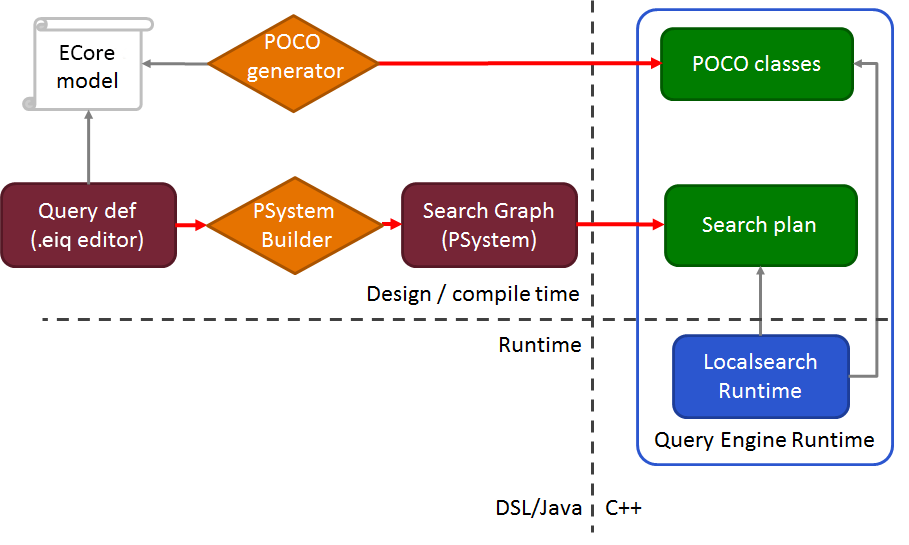
\includegraphics[width=150mm, keepaspectratio]{figures/architecture.png}
\caption{The architecture of the engine}
\label{fig:architecture}
\end{figure}

From the ECore model, the POCO generator (\sectref{GeneratedCodeStructure})
generates the \CPP{} classes. These are the classes the runtime model consists
of and the queries can be executed on.

Writing queries is supported through the \EIQ{} pattern language editor, which
provides content assist, syntax highlighting, validation and several other
features to help the user in query development.

From the query definition the search graph (called \emph{PSystem} in
\EIQ{}) gets transformed. This search graph contains every information
necessary to create the search plan. The search plan gets transformed from the
search graph to Java first, then based on this plan the actual search operations
get transformed into \CPP{} code. The available search operations and their
execution is coded in a runtime library. The assembly of the actual search plan
and it's execution gets obfuscated by generated code, the user only has to call
the appropriate generated method to get the matching elements to a specific query.

This architecture makes it so that the user has no interaction with any
localsearch related part of the application, i.e. he has to create the model,
write the queries and later on call the queries in his \CPP{} application,
everything else is handled hidden from him.
